\documentclass[letterpaper]{article}
\usepackage[margin=1in]{geometry} % Sets page size and 1-inch margins
\usepackage[svgnames,dvipsnames]{xcolor}   % For a wider range of colors

\usepackage{amsmath} % For math symbols like \to, \langle, \rangle
\usepackage{array}   % For advanced column specifications
\usepackage{tabularx}% For tables with auto-expanding columns
\usepackage{tikz}
\usetikzlibrary{
    positioning,      % For placing nodes relative to each other (e.g., below=of)
    shapes.geometric, % For shapes like ellipses
    arrows.meta,      % For advanced arrow tips (e.g., Stealth)
    decorations.pathmorphing, % For snake/squiggly lines
    calc              % For coordinate calculations
}

% --- GLOBAL STYLE DEFINITIONS FOR DFD ---
\tikzset{
    % A shape for logical connectives
    connective_node/.style={
        rectangle, rounded corners=5pt, draw=black!80, fill=black!10,
        inner sep=5pt, thick, align=center
    },
    % A shape for Introduction Rules
    intro_rule_node/.style={
        rectangle, rounded corners=5pt, draw=black!80, fill=Teal!20,
        inner sep=5pt, thick, align=center
    },
    % A shape for Elimination Rules
    elim_rule_node/.style={
        rectangle, rounded corners=5pt, draw=black!80, fill=BurntOrange!20,
        inner sep=5pt, thick, align=center
    },
    % A shape for abstract propositions
    proposition_node/.style={
        ellipse, draw=black!80, fill=Violet!15,
        inner sep=3pt, align=center
    },
    % A shape for concrete proof terms
    proof_node/.style={
        ellipse, draw=black!80, fill=Green!15,
        inner sep=3pt, align=center
    },
    % Interface ports for composition
    input_port/.style={
        circle, draw=blue!70!black, fill=blue!20,
        inner sep=2pt, minimum size=8pt
    },
    output_port/.style={
        circle, draw=ForestGreen!80!black, fill=ForestGreen!20,
        inner sep=2pt, minimum size=8pt
    },
    % Arrow styles with color
    input_arrow/.style={-Stealth, solid, thick, draw=blue!70!black},
    output_arrow/.style={double, double distance=1.5pt, -Stealth, solid, thick, draw=ForestGreen!80!black},
    proves_arrow/.style={-Stealth, decorate, decoration={snake, segment length=6pt, amplitude=1pt}, thick, draw=orange!90!black}
}

% --- Define and measure boxes to get widths for tabularx ---
\newlength{\impliesheaderwidth}
\settowidth{\impliesheaderwidth}{\textbf{Implies} : Prop $\to$ Prop $\to$ Prop}
\addtolength{\impliesheaderwidth}{1em}

\begin{document}

\begin{figure}[h!]
\centering
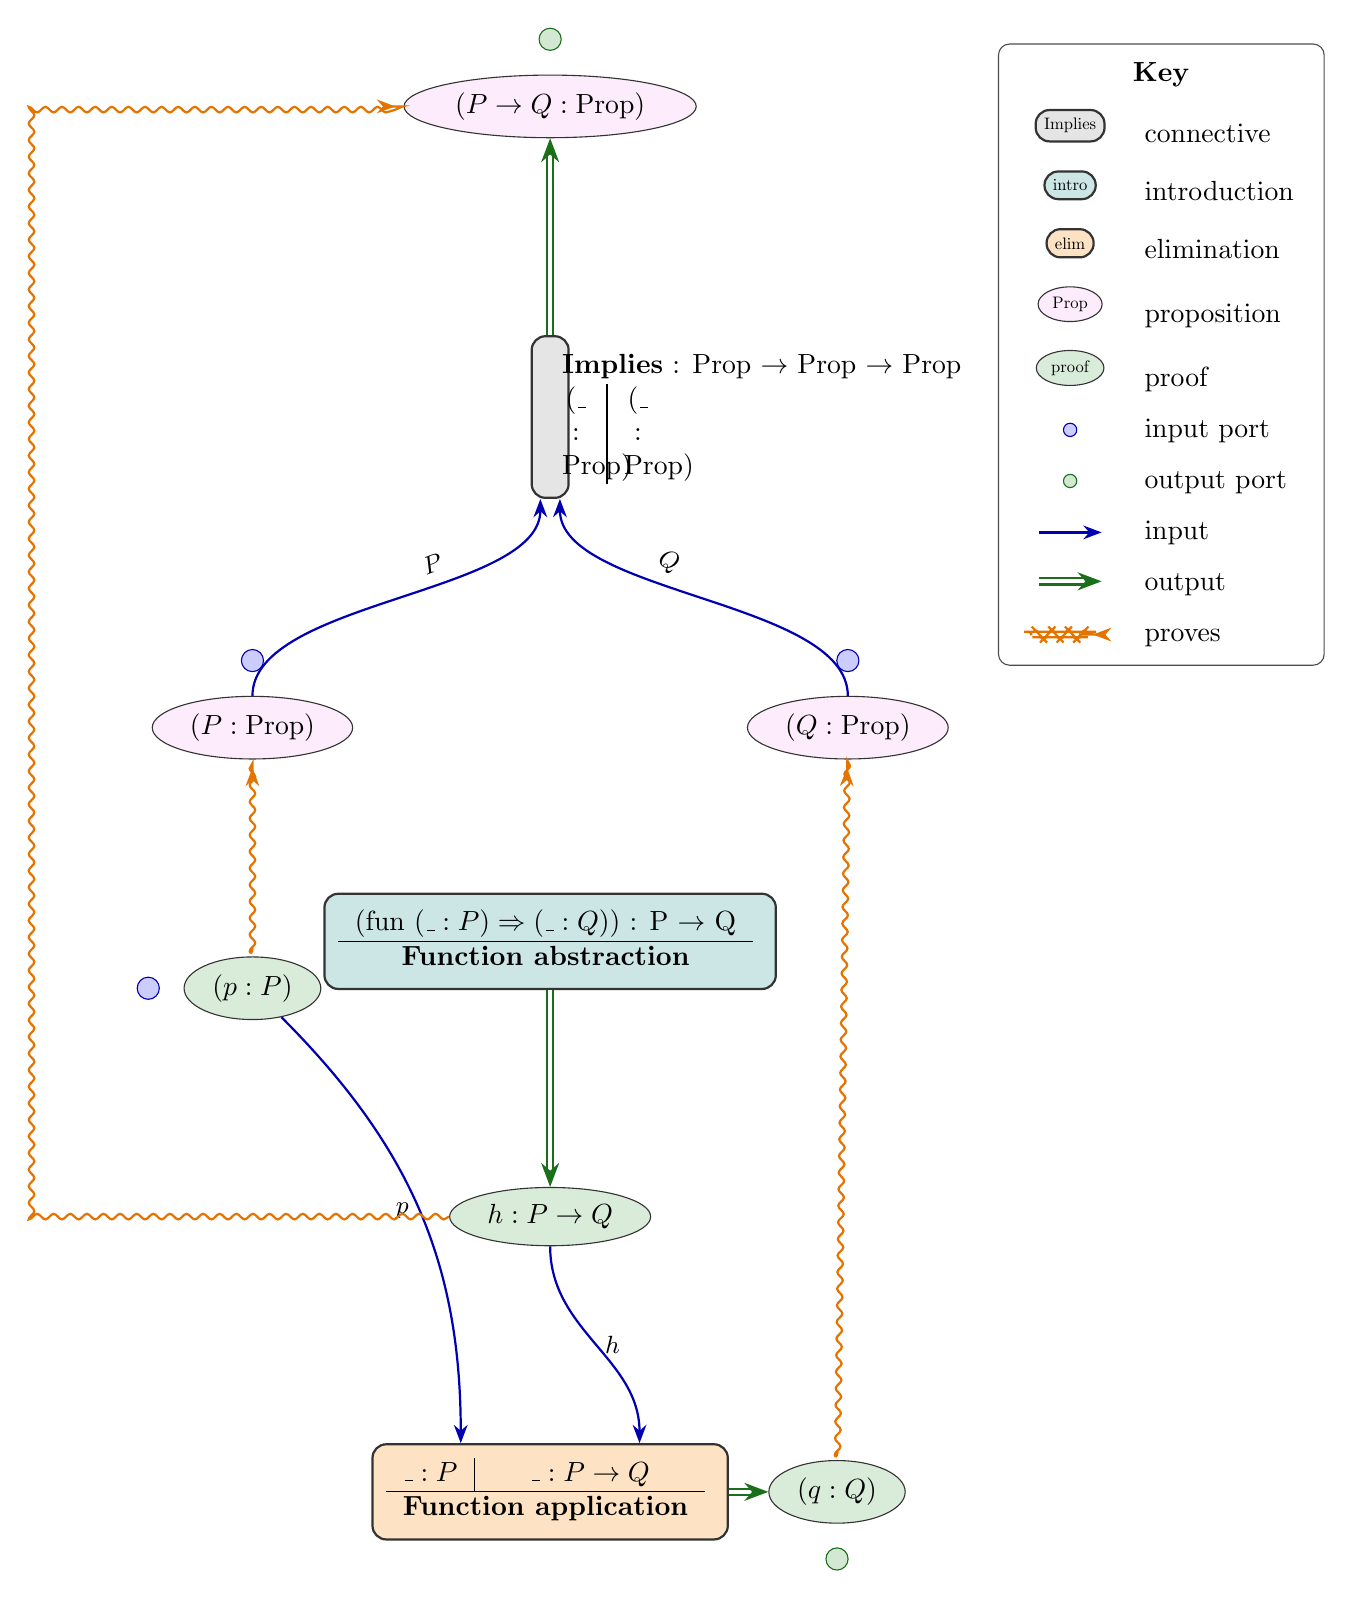
\begin{tikzpicture}[node distance=2.5cm and 2.5cm]

% --- INPUT TYPE PARAMETERS ---
\node[proposition_node] (P_prop) {$(P : \text{Prop})$};
\node[proposition_node] (Q_prop) [right=5cm of P_prop] {$(Q : \text{Prop})$};

% Input ports for type parameters
\node[input_port] (P_in_port) [above=0.3cm of P_prop] {};
\node[input_port] (Q_in_port) [above=0.3cm of Q_prop] {};

% --- CONNECTIVE LAYER ---
\node[connective_node, above=2.5cm of $(P_prop.north)!.5!(Q_prop.north)$] (implies_box) {
    \begin{tabularx}{\impliesheaderwidth}{>{\centering\arraybackslash}X|>{\centering\arraybackslash}X}
        \multicolumn{2}{c}{\textbf{Implies} : Prop $\to$ Prop $\to$ Prop} \\ \hline
        (\_ : Prop) & (\_ : Prop)
    \end{tabularx}
};

\node[proposition_node] (P_implies_Q_prop) [above=2.5cm of implies_box] {$(P \to Q : \text{Prop})$};

% Output port for result type
\node[output_port] (type_out_port) [above=0.3cm of P_implies_Q_prop] {};

% --- INTRODUCTION SECTION ---
\node[intro_rule_node, below=2.5cm of $(P_prop.north)!.5!(Q_prop.north)$] (implies_intro) {
    \begin{tabular}{c}
    $(\text{fun } (\_ : P) \Rightarrow (\_ : Q))$ : P $\to$ Q \\ \hline
    \textbf{Function abstraction}
    \end{tabular}
};

\node[proof_node] (h_P_to_Q) [below=2.5cm of implies_intro] {$h : P \to Q$};

% --- ELIMINATION SECTION ---
\node[proof_node] (p_premise) [below=2.5cm of P_prop] {$(p : P)$};

% Input port for premise
\node[input_port] (p_in_port) [left=0.3cm of p_premise] {};

% Elimination rule
\node[elim_rule_node, below=2.5cm of h_P_to_Q] (implies_elim) {
    \begin{tabular}{c|c}
    $\_ : P$ & $\_ : P \to Q$ \\ \hline
    \multicolumn{2}{c}{\textbf{Function application}}
    \end{tabular}
};

\node[proof_node] (result_Q) [right=0.5cm of implies_elim] {$(q : Q)$};

% Output port for result
\node[output_port] (q_out_port) [below=0.3cm of result_Q] {};

% --- EDGE ROUTING ---
\draw[output_arrow] (implies_box) -> (P_implies_Q_prop);
\draw[input_arrow] (P_prop.north) to[out=90, in=-90, looseness=0.7] node[pos=0.6, sloped, above, font=\small] {$P$} ($(implies_box.south west)!.5!(implies_box.south)$);
\draw[input_arrow] (Q_prop.north) to[out=90, in=-90, looseness=0.7] node[pos=0.6, sloped, above, font=\small] {$Q$} ($(implies_box.south)!.5!(implies_box.south east)$);

\draw[output_arrow] (implies_intro) -> (h_P_to_Q);

\draw[input_arrow] (p_premise) to[out=-45, in=90] node[pos=0.5, left, font=\small] {$p$} ($(implies_elim.north west)!.5!(implies_elim.north)$);
\draw[input_arrow] (h_P_to_Q) to[out=-90, in=90] node[pos=0.5, right, font=\small] {$h$} ($(implies_elim.north)!.5!(implies_elim.north east)$);

\draw[output_arrow] (implies_elim.east) -> (result_Q.west);

% Proves arrows
\draw[proves_arrow, shorten <=3pt, shorten >=3pt] (p_premise) -> (P_prop);
\draw[proves_arrow, shorten <=3pt, shorten >=3pt] (result_Q) -> (Q_prop);

% Main "proves" arc
\coordinate (outset_point) at ($(P_prop.west)+(-1.5cm,0)$);
\draw[proves_arrow, shorten >=3pt] (h_P_to_Q.west) -- (outset_point |- h_P_to_Q.west) -- (outset_point |- P_implies_Q_prop.west) -- (P_implies_Q_prop.west);

% --- LEGEND ---
\node (legend) [draw=black!70, rounded corners, inner sep=5pt, above right=0.5cm and 1cm of Q_prop] {
    \begin{tabular}{cl}
    \multicolumn{2}{c}{\textbf{Key}} \\[1.5ex]
    \tikz{\node[connective_node, scale=0.6] {Implies};} & connective \\[1.5ex]
    \tikz{\node[intro_rule_node, scale=0.6] {intro};} & introduction \\[1.5ex]
    \tikz{\node[elim_rule_node, scale=0.6] {elim};} & elimination \\[1.5ex]
    \tikz{\node[proposition_node, scale=0.6] {Prop};} & proposition \\[1.5ex]
    \tikz{\node[proof_node, scale=0.6] {proof};} & proof \\[1.5ex]
    \tikz{\node[input_port, scale=0.6] {};} & input port \\[1.5ex]
    \tikz{\node[output_port, scale=0.6] {};} & output port \\[1.5ex]
    \tikz{\draw[input_arrow] (0,0.1) -- (0.8,0.1);} & input \\[1.5ex]
    \tikz{\draw[output_arrow] (0,0.1) -- (0.8,0.1);} & output \\[1.5ex]
    \tikz{\draw[proves_arrow] (0,0.1) -- (0.8,0.1);} & proves \\
    \end{tabular}
};

\end{tikzpicture}
\caption{Modular Implies connective with composition interfaces. Input ports accept type parameters and proof terms. The function abstraction creates the implication type, while function application eliminates it. Output ports provide results for composition with other operators.}
\label{fig:implies_modular}
\end{figure}

\end{document}

\end{document>